\graphicspath{{img/chapter_2/}}



\chapter{A Primer on Compact Objects}
\label{chapter:compactobjects}

% \begin{synopsis}
% Introduce COs, formation, structure etc...  
% \end{synopsis}
%%%%%%%%%%%%%%%%%%%%%%%%%%%%%%%%%%%%%
%%%%%%%%%%%%%%%%%%%%%%%%%%%%%%%%%%%%%
%%%%%%%%%%%%%%%%%%%%%%%%%%%%%%%%%%%%%

Within the cores of stars exists a delicate balance between the gravitational force of its mass wanting to collapse in on itself, and the outward pressure generated by thermonuclear fusion of light elements. This fusion process begins with the burning of hydrogen to form helium. Eventually, the hydrogen is depleted, allowing gravity to temporarily overcome the outward pressure leading to the core contracting. As this occurs, the gravitational potential energy is converted to thermal energy and the core eventually becomes hot enough to facilitate helium burning. 

This cycle continues as heavier and heavier elements are formed within the ever-increasingly hot stellar core.
If the star is heavy enough, iron will eventually be formed from the burning of silicon. As the fusion of iron nuclei is an endothermic process, it will not occur spontaneously. Whatever the mass of the star, eventually it will no longer be able to support the fusion of these heavier elements. Without a sufficient fuel source, the core will collapse under its own gravity leading to the death of the star.  

What comes after this depends on the mass of the progenitor stars. Very light stars, $\lesssim 0.5 \Msun$, have lifetimes much longer than the age of the universe, and so are uninteresting to our current discussion. Moderately heavy stars, $1\Msun\lesssim \Mstar \lesssim 8\Msun$, will continue burning fuel until the outer layers of the star are dispersed as it expands, leaving a carbon-oxygen (CO) core. The core will begin to collapse until the Fermi degeneracy of the ultrarelativistic electrons is great enough to reestablish equilibrium, resulting in a White Dwarf (WD).

Heavy stars, $\gtrsim 8\Msun$, spectacularly end their lives in a type-II supernova event. This occurs when the core of the star exceeds the Chandrashekhar mass of $1.4\Msun$, which cannot be supported by electron degeneracy pressure. The core itself will then collapse, leading to a shockwave that ejects the majority of the mass of the star. All that will remain is an extremely dense core supported by neutron degeneracy pressure, a Neutron Star (NS). If the star was so massive that the gravitational forces overcome even the neutron degeneracy pressure, then the core collapses into a black hole. 

These three stellar corpses (white dwarfs, neutron stars, and black holes) are collectively known as compact objects, as they have masses similar to or larger than our Sun, compressed into much smaller bodies with significantly larger surface gravities. These objects do not have a source of fuel, and spend the rest of their lives cooling down. For the remainder of this thesis, we will only be interested in white dwarfs and neutron stars and refer to these collectively as compact objects, excluding black holes from this term. 

This chapter is dedicated to discussing the structure and composition of these objects\footnote{As this work is written by a particle physicist, I wish to apologise to my astrophysics colleagues for what is to come.}.


%%%%%%%%%%%%%%%%%%%%%%%%%%%%%%%%%%%%%
%%%%%%%%%%%%%%%%%%%%%%%%%%%%%%%%%%%%%
%%%%%%%%%%%%%%%%%%%%%%%%%%%%%%%%%%%%%
\section{Structure Equations from General Relativity}
%%%%%%%%%%%%%%%%%%%%%%%%%%%%%%%%%%%%%
%%%%%%%%%%%%%%%%%%%%%%%%%%%%%%%%%%%%%

The highly dense matter comprising neutron stars and white dwarfs leads to extremely strong gravitational fields being produced by the stars. As such, modeling the structure of these objects falls into the domain of General Relativity (GR). Here we review the structure of static, spherically symmetric stars. 

The assumption that the mass distribution of the star is spherically symmetric leads to the metric taking the form
\begin{equation}
    ds^2 = -d\tau^2 = -B(r) dt^2 + A(r) dr^2 + r^2 d\Omega^2,
\end{equation}
with $d\tau$ the proper time interval, and $A(r),\;B(r)$ are functions only of the radial coordinate and are often written as 
\begin{equation}
    A(r) = e^{2\Lambda(r)},\quad B(r) = e^{2\Phi(r)}.
\end{equation}
These functions are subject to the condition that at distances far from the star space-time becomes flat, leading to the boundary conditions 
\begin{equation}
    \lim_{r\rightarrow \infty} A(r) = \lim_{r\rightarrow \infty} B(r)  = 1.
\end{equation}

The matter that comprises the star is modeled as a perfect fluid, meaning we are neglecting any shear stresses and energy transport within the star. Such a fluid is described by its pressure $P(r)$, density $\rho(r)$, and number density, $n(r)$, as well as the 4-velocity of the fluid $u^\mu(r)$. Being a static fluid, the only non-zero component of this velocity is the time component, which is fixed through $g_{\mu\nu}u^\mu u^\nu = -1$ to be $u^t = 1/\sqrt{B(r)}$.
These quantities are then used to construct the stress-energy tensor for the star, which takes the form
\begin{equation}
    T^{\mu\nu} = (\rho + P)u^\mu u^\nu + P g^{\mu\nu}.
\end{equation}
The microphysics underlying the matter interactions are encoded in an equation of state (EoS) that relates the various thermodynamic quantities. This is typically given by expressing the pressure as a function of the density, $P(\rho)$. It is often more convienient to parameterise the EoS by the number density of baryons, $n_b$, and the entropy per baryon, $s$, such that 
\begin{equation}
    P=P(n, s), \quad \rho = \rho(n, s).
\end{equation}
The dependence on $s$ turns out to be trivial in most scenarios involving compact objects, such as those considered here. The pressure in these stars arises from the degeneracy of the nucleons in NSs or the electrons in WDs, rather than from the thermal motion of the constituents that will be frozen out at low temperatures. This is the case for temperatures much lower than the Fermi energy of the system, with typical values of $E_F \sim 10\MeV$ in NSs or $\sim 1 \MeV$ in WDs, corresponding to temperatures of $T_\star\sim 10^{11}\K$ and $\sim 10^{10}\K$ respectively. As these stars are expected to cool well below these temperatures quickly after formation, the entropy can be taken to be zero throughout the star. This allows us to reduce the two-parameter EoS to a simpler one-parameter one,
\begin{equation}
    P=P(n_b, s = 0) = P(n_b), \quad \rho = \rho(n_b, s=0) = \rho(n_b).\label{eq:1_param_EoS}
\end{equation} 


The structure of the star is therefore determined by the quantities $A(r)$, $B(r)$, $P(r)$, $\rho(r)$, and $n_b(r)$. This system is determined by applying the Einstein field equations, $G^{\mu\nu} = 8\pi T^{\mu\nu}$, together with the conservation of energy-momentum, $T^{\mu\nu}_{\quad;\nu}=0$, the EoS relations Eqs.~\ref{eq:1_param_EoS}, and the appropriate boundary conditions. The structure equations that come out of this analysis were first discovered concurrently by Tolman~\cite{Tolman:1939jz_StaticSolutionsEinstein} and by Oppenheimer and Volkoff~\cite{Oppenheimer:1939ne_MassiveNeutronCores}, and so are known as the TOV equations. They take the form
\begin{align}
    \frac{dP}{dr} &= -\rho(r) c^2  \left[ 1 + \frac{P(r)}{\rho(r) c^2} \right]\frac{d\Phi}{dr},\label{eq:TOV_1}\\
    \frac{d\Phi}{dr} & = \frac{G M(r)}{c^2 r^2} \left[ 1 + \frac{4\pi r^3 P(r)}{M(r)c^2} \right] \left[ 1 - \frac{2 G M(r)}{c^2 r}\right]^{-1}\label{eq:TOV_2},\\
    \frac{dB}{dr} & = 2B(r) \frac{d\Phi}{dr},\label{eq:TOV_3}
\end{align}
where $M(r)$ is related to the metric factor $A(r)$ through
\begin{equation}
    A(r) = \left[ 1 - \frac{G M(r)}{c^2 r} \right]^{-1},
\end{equation}
and is interpreted as the mass contained within a radius $r$. It obeys the mass equation 
\begin{equation}
    \frac{dM}{dr} = 4\pi r^2 \rho(r),\quad M(0) = 0,
    \label{eq:mass_equation_TOV}
\end{equation}
that arises from the $\mu = \nu = 0$ component of the Einstein field equiations. 
These equations are the general relativistic versions of the hydrostatic equilibrium equations of regular stellar structure, with Eq.~\ref{eq:TOV_1} reducing to the familiar 
\begin{equation}
    \frac{dP}{dr} = -\frac{GM(r)}{r^2}\rho(r),
\end{equation}
in the Newtonian limit, $GM(r)/c^2 r \ll 1$.

The radius of the star, $\Rstar$, is identified as the point at which the pressure and density vanish, $P(\Rstar) = \rho(\Rstar) = 0$. In the region outside the star, $r>\Rstar$, the total mass remains constant at the total mass of the star, $M(r \geq  \Rstar) = \Mstar$, and so the only non-trivial structure functions are the metric factors. Solving Eq.~\ref{eq:TOV_3} with $P(r)=0$ and constant $M(r)$ for $B(r)$ becomes elementary while the result for $A(r)$ is trivial, leaving us with
\begin{equation}
    A(r) = \left[ 1 - \frac{G \Mstar}{c^2 r} \right]^{-1}, \quad B(r) = 1 - \frac{G \Mstar}{c^2 r} ,\quad\mathrm{for}\;r > \Rstar,
\end{equation}
and the metric reduces to the familiar Schwarzschild metric outside the star. 
Continuity of the metric at $r= \Rstar$ enforces a second boundary condition for $B(r)$,
\begin{equation}
    B(\Rstar) = 1 - \frac{G \Mstar}{c^2 \Rstar}.
    \label{eq:B_boundary_condition}
\end{equation}

The final boundary condition required is the central pressure $P(0) = P_c$, or equivalently the central density/baryon number density. This is the only free parameter in the system and hence, for a given EoS, uniquely determines the stellar structure. All stars generated by an EoS can therefore be represented as a one-parameter sequence, typically represented as the mass-radius relation for the model. 

Given all the above, we can write a simple recipe for constructing a model of a compact object:
\begin{enumerate}
    \item Select an EoS to describe the constituent matter.
    \item Specify the central pressure of the star, $P_c$.
    \item Integrate the coupled system of differential equations \ref{eq:TOV_1}, \ref{eq:TOV_2}, \ref{eq:mass_equation_TOV} from the centre of the star outward until the pressure vanishes.
    \item Use the boundary condition Eq.~\ref{eq:B_boundary_condition} to normalise the metric function $B(r)$. 
\end{enumerate}
In general, additional quantities will be present in the EoS, such as chemical potentials or the speed of sound, that may be subject to additional constraints. These quantities will need to be calculated at each step of the integration alongside the other EoS quantities. 

%%%%%%%%%%%%%%%%%%%%%%%%%%%%%%%%%%%%%
%%%%%%%%%%%%%%%%%%%%%%%%%%%%%%%%%%%%%
%%%%%%%%%%%%%%%%%%%%%%%%%%%%%%%%%%%%%
\section{White Dwarfs}
%%%%%%%%%%%%%%%%%%%%%%%%%%%%%%%%%%%%%
%%%%%%%%%%%%%%%%%%%%%%%%%%%%%%%%%%%%%
%%%%%%%%%%%%%%%%%%%%%%%%%%%%%%%%%%%%%

The fate of main sequence stars of mass below $\Mstar \lesssim 8 \Msun$ is to end their life cycles as a white dwarf. Consequently, these compact stellar remnants, which are supported against gravitational collapse by electron degeneracy pressure, are the most abundant stars in the Galaxy ($\gtrsim 90\%$). They are born at very high temperatures and cool down over billions of years. Observations of the coldest WDs therefore contain information on the star formation history of the Galaxy.

The vast majority of observed WDs are composed primarily of carbon and oxygen, plus small traces of elements heavier than helium. 
At the extremely high densities found in WDs $\sim10^6-10^{10}\g\cm^{-3}$, electrons are strongly degenerate and determine the WD equation of state (EoS) and internal structure.  The stellar core resembles a Coulomb lattice of ions surrounded by degenerate electrons, which implies that the WD core is isothermal and a very good thermal conductor. 
The degenerate core is enclosed by a thin envelope that accounts for $\lesssim 1\%$  of the total mass~\cite{Fontaine_apr_Potentialwhitedwarf}. 

The outer layers form an atmosphere that is rich in lighter elements such as hydrogen or helium, where the exact composition depends on the evolution of the WD progenitor and changes as the WD cools. 
This atmosphere is non-degenerate and extremely opaque to radiation, with an EoS that is subject to finite temperature effects. 

%%%%%%%%%%%%%%%%%%%%%%%%%%%%%%%%%%%%%
%%%%%%%%%%%%%%%%%%%%%%%%%%%%%%%%%%%%%
\subsection{The FMT Equation of State}
%%%%%%%%%%%%%%%%%%%%%%%%%%%%%%%%%%%%%
%%%%%%%%%%%%%%%%%%%%%%%%%%%%%%%%%%%%%


In the limit of zero temperature, the simplest way to obtain the WD EoS is to assume an ideal Fermi gas of degenerate electrons, for a WD that is primarily composed of a single element. Corrections to the non-interacting electron picture were introduced early by Salpeter~\cite{Salpeter:1961zz_nov_Energypressurezerotemperature}. By introducing the Wigner-Seitz (WS) cell approximation and assuming point-like nuclei, Salpeter obtained an analytical EoS that accounts for interactions between electrons and ions as well as other Coulomb corrections. These corrections, in general, depend on the chemical composition of the star. 

More recently, it has been shown that the treatment of matter at high pressures presented by Feynman, Metropolis and Teller~\cite{Feynman:1949zz_Equationsstateelements} can be extended to consistently take into account weak interactions and relativistic effects \cite{Rotondo:2009cr_RelativisticThomasFermitreatment,Rotondo:2011zz_RelativisticFeynmanMetropolisTellertheory}, and incorporates Coulomb corrections in a more natural manner than the Salpeter EoS. The resulting Feynman-Metropolis-Teller (FMT) EoS is obtained by considering a relativistic Thomas-Fermi model within Wigner-Seitz cells of radius $R_{\mathrm WS}$. 
For degenerate, relativistic, electrons, the equilibrium condition is that the Fermi energy, $E_e^F$, is constant within the cell,
\begin{equation}\label{eq:rel_equil}
E_e^F=\sqrt{(p_e^F)^2+m_e^2}-m_e-eV(r) = \rm{constant},
\end{equation}
where $V(r)$ is the Coulomb potential inside the cell, $p_e^F$ is the electron Fermi momentum, $m_e$ is the electron mass and $e$ is the electric charge. To obtain an integrable solution for the energy density near the origin, it is necessary to introduce a finite size for the nucleus, with radius $ R_c = \Delta\lambda_{\pi} Z^{1/3}$, 
where $\lambda_\pi$ is the pion Compton wavelength, $\Delta \approx (r_0 /\lambda_\pi)(A/Z)^{1/3}$, $Z$ is the proton number, $A$ is the atomic mass, and $r_0$ is an empirical constant $\sim 1.2\;\text{fm}$. The proton and electron number densities inside the cell are then given by
\begin{align}
    n_p &=  \frac{(p^F_p)^3}{3\pi^2} =\frac{3Z}{4\pi R_c^3}\theta( R_c - r ) = \frac{3}{4\pi} \left( \frac{1}{\Delta \lambda_\pi} \right)^3 \theta(R_c -r), \label{eq:prot_dens_FMT}\\
    n_e &= \frac{(p^F_e)^3}{3\pi^2} = \frac{1}{3\pi^2}\left[ \hat{V}^2(r) + 2m_e \hat{V}(r)\right]^{3/2},\label{eq:elec_dens_FMT}\\
    \hat{V}(r) &= eV(r) + E_e^F. \label{eq:vhat}
\end{align}
The Coulomb potential satisfies the Poisson equation 
\begin{equation}
    \nabla^2 V(r) = -4\pi e[n_p(r) - n_e(r)],
    \label{eq:poisson_WS_cell}
\end{equation} 
with requiring global charge neutrality of the cell enforcing the boundary conditions
\begin{equation}
    \left.\frac{dV}{dr}\right|_{r = R_\mathrm{WS}} = V(R_\mathrm{WS}) = 0.
\end{equation}
In practice, it is beneficial to work with dimensionless quantities, and so we define $x = r/\lambda_\pi$ and $\chi(r) = r\hat{V}(r)$, such that $x_c = R_c/\lambda_\pi$ and $x_{\mathrm WS} = R_{\mathrm WS}/\lambda_\pi$.
Using these expressions results in the relativistic Thomas-Fermi equation
\begin{equation}
    \frac{1}{3x}\frac{d^2\chi}{dx^2} = -\frac{\alpha_{\mathrm{EM}}}{\Delta^3}\theta(x_c -x) + \frac{4\alpha_\mathrm{EM}}{9\pi}\left[ \frac{\chi^2(x)}{x^2} + 2\frac{m_e}{m_\pi}\frac{\chi(x)}{x}\right]^{3/2},\label{eq:FMT_DE}
\end{equation}
with the boundary conditions
\begin{equation}
    \chi(0) = 0, \qquad
    \left. \frac{d\chi}{dx}\right|_{x_{\mathrm{WS}}} = \frac{\chi(x_{\mathrm WS})}{x_{\mathrm{WS}}}. \label{eq:TF_bc}
\end{equation}

By solving these equations, we can obtain the relevant thermodynamic quantities, namely the electron and proton number densities, electron chemical potential, and the energy and pressure of the cell. The electron chemical potential is obtained by evaluating Eq.~\ref{eq:rel_equil} at the cell radius, noting that the Coulomb potential must vanish there, which results in the usual expression\footnote{We use the symbol $\varepsilon_{F,i}$ to represent the chemical potential minus the mass of a particle species $i$, reserving $\mu_{F,i}$ for the full chemical potential.}
\begin{equation}
    \varepsilon_{F,e} = \sqrt{(p_e^F)^2+m_e^2}-m_e.\label{eq:mufe}
\end{equation}
The energy and pressure of the cell can then be obtained following the analysis presented in~ref.~\cite{Rotondo:2011zz_RelativisticFeynmanMetropolisTellertheory}. The cell energy gains contributions from the nuclear mass, electron kinetic energy, and Coulomb interactions, such that
\begin{align}
    E_\mathrm{tot} & = M_N + E_k + E_C,\label{eq:total_E_cell}\\
    E_k & = \int_0^{R_{\mathrm WS}}4\pi r^2 [\mathcal{E}_e(r) - m_e n_e(r)]\;dr,\label{eq:kinetic_E_cell}\\
    E_C & = \frac{1}{2}\int_{R_c}^{R_{\mathrm WS}}4\pi r^2 e[n_p(r) - n_e(r)]V(r)\;dr,\label{eq:Coulomb_E_cell}
\end{align}
where 
\begin{equation}
    \mathcal{E}_e(r) = \frac{1}{\pi^2}\int_0^{p_e^F}p^2\sqrt{p^2 + m_e^2}\;dp,
\end{equation}
is the electron energy density, and  $M_N$ is the mass of the nucleus. The energy density of the cell is then simply
\begin{equation}
    \rho_\mathrm{WS} = \frac{E_\mathrm{tot}}{V_\mathrm{WS}},
\end{equation} 
where $V_\mathrm{WS} = 4\pi R_\mathrm{WS}/3$ is the volume of the WS cell. 
The only contribution to the internal cell pressure comes from the electrons,
\begin{equation}
    P_e(r) = \frac{1}{3\pi^2}\int_0^{p_e^F}\frac{p^4}{\sqrt{p^2+m_e^2}}\;dp,
\end{equation}
with the total pressure of the cell being $P_\mathrm{tot} = P_e(R_{\mathrm WS})$.
Finally, the EoS is then obtained by solving Eq.~\ref{eq:FMT_DE} for various cell radii, yielding a relation between $E_\mathrm{tot}$ and $P_\mathrm{tot}$ parameterised by the radius of the Wigner-Seitz cell. 


\begin{table}[t]
  \centering
    \begin{tabular}{|l|l|l|l|l|} % <-- Changed to S here.
    \hline
      \textbf{EoS} & \textbf{WD}$_\mathbf{1}$  & \textbf{WD}$_\mathbf{2}$&\textbf{WD}$_\mathbf{3}$ &\textbf{WD}$_\mathbf{4}$\\
      \hline
     $\rho_c\,[\g\cm^{-3}]$ &  $1.47\times 10^{6}$ & $3.84\times 10^{7} $ & $3.13\times 10^{8}$ & $2.31\times 10^{10}$\\
     $\Mstar\,[M_\odot]$ & $0.440$ &  $1.000 $ & $1.252$ & $1.384$\\
     $\Rstar\,[\km]$ & $9.39\times 10^{3}$ &  $5.38\times 10^{3}$ & $3.29\times 10^3$ & $1.25\times 10^3$\\
     $\vesc(\Rstar) \, [\km/\s]$ & $3.72\times 10^{3}$ & $7.03\times 10^{3}$ & $1.01\times 10^{4}$ & $1.71\times 10^{4}$ \\
      \hline
    \end{tabular}
  \caption{Four configurations for white dwarfs composed of carbon, with an FMT EoS. Shown are the central densities, $\rho_c$, stellar mass $\Mstar$ and radius $\Rstar$, and escape velocity at the edge of the WD, $\vesc$. }
    \label{tab:WDs}
\end{table}
 


Different WD configurations can be obtained, assuming a non-rotating spherically symmetric star, by solving the
Tolman-Oppenheimer-Volkoff (TOV) equations~\cite{Tolman:1939jz_StaticSolutionsEinstein,Oppenheimer:1939ne_MassiveNeutronCores} coupled to the FMT EoS with different initial conditions for the pressure at the centre of the star. In Fig.~\ref{fig:WDradprofs} we show radial profiles for $n_e$ (top left), $\muFe$ (top right), and escape velocity $\vesc$ (bottom) for the carbon WDs in Table~\ref{tab:WDs}. Note that the difference in radius between the lightest and heaviest WD in Table~\ref{tab:WDs} spans almost one order of magnitude, while the electron number densities in the core can vary up to 4 orders of magnitude (see top left panel). As expected, electrons are more degenerate in more compact WDs and become relativistic (see top right panel). The escape velocity can reach ${\mathcal{O}}(0.1\,c)$ at the interior of the most compact WDs, while for very low mass WDs 
it can be as low as $\sim0.003\,c$. 

\begin{figure}[!t]
    \centering
    \includegraphics[width = 0.495\textwidth]{ne_prof.pdf}  
    \includegraphics[width = 0.495\textwidth]{muFe_prof.pdf}  
    \includegraphics[width = 0.67\textwidth]{vesc_prof.pdf}
    \caption{Electron number density (top left), chemical potential (top right), and escape velocity (bottom) radial profiles for the carbon WDs with FMT EoS in Table~\ref{tab:WDs}. The radial distance of each profile has been normalised to the radius of the star.}
    \label{fig:WDradprofs}
\end{figure}


The mass-radius relations obtained from a zero-temperature EoS begin to deviate from observations for low-mass WDs. 
To address this discrepancy, finite temperature effects can be introduced to the EoS~\cite{deCarvalho:2013rea_Relativisticfeynmanmetropolistellertreatment}. 
The extension to finite temperatures is made by reintroducing the temperature dependence in the Fermi-Dirac
distributions. Now, the electron chemical potential is no longer simply the Fermi energy of the system due to thermal corrections. Define the finite temperature Fermi-Dirac integrals of degree $s$ as
\begin{equation}
    F_s (\eta, \beta) = \int_0^\infty \frac{t^s\sqrt{1 + (\beta/2)t}}{1 + e^{t - \eta}}dt,
\end{equation}
where we define the dimensionless quantities 
\begin{align}
    t & = \frac{E_e - m_e}{\Tstar},\\
    \eta & = \frac{\varepsilon_{F,e}}{\Tstar},\\
    \beta & = \frac{\Tstar}{m_e},
\end{align}
for a star at temperature $\Tstar$. The Thomas-Fermi equilibrium condition within the WS cell is now given by 
\begin{equation}
    \varepsilon_{F,e}(r) - e V(r) = \Tstar \eta(r) - e V(r) = \mathrm{constant},
\end{equation}
with the Coulpmb potential vanishing at the boundary of the cell as before. We now make the change of variables into the dimensionless quantities $\chi/r = \varepsilon_{F,e} / (\hbar c)$ and $x = x/x_\mathrm{WS}$ so that the Poisson equation~\ref{eq:poisson_WS_cell} becomes
\begin{align}
    \frac{d^2 \chi}{dx^2} &= -4 \pi \alpha_\mathrm{EM} x \left( \frac{3}{4\pi \Delta^3} \theta(x_c - x) - \frac{\sqrt{2}}{\pi^2} \left( \frac{m_e}{m_\pi} \right)^2\left[ F_{1/2}(\eta, \beta) + \beta  F_{3/2}(\eta, \beta) \right] \right),\\
    \eta(x) & = \left(\frac{1}{\lambda_\pi \Tstar}\right)\frac{\chi(x)}{x},
\end{align}
with the same boundary conditions as in Eq.~\ref{eq:TF_bc}.

The total energy of the cell remains very similar to the zero-temperature case, the main differences being it gains a contribution from the thermal motion of the nucleus, 
\begin{equation}
    E_\mathrm{th} = \frac{3}{2}\Tstar,
\end{equation} 
and that the electron energy density is now given by
\begin{equation}
    \mathcal{E}_e = m_e n_e + \frac{\sqrt{2}}{\pi^2} m_e^4 \beta^{5/2} \left[ F_{3/2}(\eta, \beta) + \beta F_{5/2}(\eta, \beta) \right].
\end{equation}

The pressure of the cell will now gain contributions from the motion of the nucleus as well as the electron, such that the total pressure is
\begin{align}
    P_\mathrm{tot} & = P_N + P_e,\\
    P_N & = \frac{2}{3}\frac{E_\mathrm{th}}{V_\mathrm{WS}} = \frac{\Tstar}{V_\mathrm{WS}},\\
    P_e & = \frac{2^{3/2}}{3\pi} me^4 \beta^{5/2}\left[  F_{3/2}(\eta(x_\mathrm{WS}), \beta) + \beta F_{5/2}(\eta(x_\mathrm{WS}), \beta)  \right].
\end{align}

In Fig.~\ref{fig:WD_mass_radius} we show the Mass-Radius relations obtained from the zero temperature FMT EoS together with several finite temperature configurations. As can be seen, the deviations from the zero temperature approximation begin at rather high temperatures, $\Tstar\gtrsim 10^7\K$, for masses $\lesssim 0.6 \Msun$. Additionally, we show observations of WDs from the Gaia early data release 2 (EDR2) report~\cite{GentileFusillo_feb_GaiaDataRelease} as the blue dots. As mentioned above, the Mass-Radius relation seen from these observations significantly deviates from the zero temperature EoS as low masses. Note that while not represented in this figure, the temperature of the WDs increases in a similar gradient as would be expected from the FMT EoS.

Given the non-linear nature of the differential equations that describe the FMT EoS (both at zero and finite temperatures), solving the system is a numerically challenging task. As there are no publically available resources to help solve these systems, a significant amount of time was put into solving this problem. As such, we have outlined in Appendix~\fixMV{ADD THIS APPENDIX} the method employed in numerically solving the differential equations. 


\begin{figure}[!ht]
    \centering
    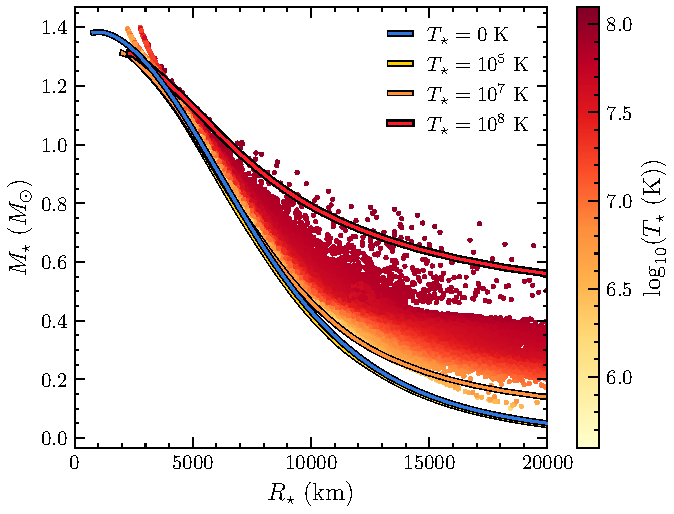
\includegraphics{WD_mass_radius.pdf}
    \caption{Mass-Radius relation of WDs calculated from the FMT EoS in the zero temperature approximation (dark blue), at $10^{5}\K$ (yellow), $10^{7}\K$ (orange), and $10^{8}\K$ (red), together with observed WDs from Gaia EDR2 observations~\cite{GentileFusillo_feb_GaiaDataRelease} (light blue dots).}
    \label{fig:WD_mass_radius}
\end{figure}

%%%%%%%%%%%%%%%%%%%%%%%%%%%%%%%%%%%%%
%%%%%%%%%%%%%%%%%%%%%%%%%%%%%%%%%%%%%
\subsection{Observational Status}
%%%%%%%%%%%%%%%%%%%%%%%%%%%%%%%%%%%%%
%%%%%%%%%%%%%%%%%%%%%%%%%%%%%%%%%%%%%

%%%%%%%%%%%%%%%%%%%%%%%%%%%%%%%%%%%%%
%%%%%%%%%%%%%%%%%%%%%%%%%%%%%%%%%%%%%
%%%%%%%%%%%%%%%%%%%%%%%%%%%%%%%%%%%%%
\section{Neutron Stars}
%%%%%%%%%%%%%%%%%%%%%%%%%%%%%%%%%%%%%
%%%%%%%%%%%%%%%%%%%%%%%%%%%%%%%%%%%%%
%%%%%%%%%%%%%%%%%%%%%%%%%%%%%%%%%%%%%

\commMV{Add some intro remarks}

The internal structure of an NS is significantly more complicated than that of a WD. Broadly speaking, an NS can be divided into five main regions. Working from the outside in, these are:

\subsubsection*{Atmosphere}
The atmosphere is an extremely thin layer of plasma that makes up less than 1\% of the NS mass. However, it plays an extremely important role as the observed spectrum radiation emitted by the star must pass through this star. This radiation contains valuable information about various properties of the star.

\subsubsection*{Outer Crust}
The outer crust is the thin layer of ionized Iron-56 nuclei that extends down until the density reaches the neutron drip point, $\rho_\star = \rho_\mathrm{ND} \sim 4.3\times 10^{11}\g\cm^{-3}$. This is the density at which neutrons begin to drip from the nuclei as their chemical potentials approach zero. The ionized electrons form a non-relativistic but degenerate gas, with their chemical potentials increasing as the density increases. This leads to the ``neutronisation'' of the nuclei as the beta-capture of electrons by protons increases.

\subsubsection*{Inner Crust}
The density within the inner crust spans the range between $\rho_\mathrm{ND}\lesssim \rho_\star \lesssim 0.5\rho_0$, with $\rho_0 \sim 2.8\times 10^{14}\g\cm^{-3}$ the nuclear saturation density (i.e. the density of nuclear matter). Here, the neutrons that have dripped from the nuclei will potentially form a superfluid. Towards the crust-core boundary, the nuclear lattice begins taking on interesting topological structures that are distinguished by the configuration of the voids in the lattice. These are known as the so-called \textit{pasta phases} of nuclear matter:
\begin{itemize}
    \item 2D void cylinders creating spaghetti structures of nuclei
    \item Planar voids with slabs of nuclei forming lasagna sheets
    \item 3D cylindrical voids leading to thin 2D cylinders of nuclear ziti
    \item 3D spherical voids enclosed by ravioli
    \item 2D circular voids in sheets of Swiss cheese
\end{itemize}
Eventually, the nuclear matter becomes a uniform medium\footnote{The nuclear marinara sauce, if you will}. 

\subsubsection*{Outer Core}
Once densities go above $0.5\rho_0$, the nuclear clusters will dissolve into a homogenous fluid that is composed of neutrons, protons, electrons, and muons known as $npeu$ matter. The relative abundances of the species, $Y_i=n_i/n_b$, are dictated by the conditions of electrical neutrality and beta-equilibrium.
Charge neutrality dictates that the abundances of the charged particles obeys
\begin{equation}
    Y_p = Y_e + Y_\mu,
\end{equation}
while beta-equilibrium refers to the balance between the weak decays of neutrons and the electron/muon capture by the protons,
\begin{gather}
    n \rightarrow p + \ell^- +\bar{\nu}_\ell,\\
    p + \ell^- \rightarrow n + \nu_\ell,
\end{gather}
with $\ell = e, \mu$. Muons will begin to replace electrons in these reactions once the electron chemical potential exceeds the mass of the muon, $\mu_{F,e} \gtrsim m_\mu = 105.7\MeV$. As the species are all degenerate, muons cannot decay into electrons, imposing the constraint 
\begin{equation}
    \mu_{F,e} = \mu_{F,\mu},
\end{equation}
on the chemical potentials. The outer core region ends once the density reaches $\rho_\star \sim 2\rho_0$, and we transition into the inner core.

\subsubsection*{Inner Core}
The densities within the inner cores of NSs extend between $2\rho_0 \lesssim \rho_\star \lesssim (10-15)\rho_0$ and are hence a mystery to this day. As the density exceeds well above any material that can be produced in a laboratory, the exact composition of this region is unknown and depends on the equation of state one adopts to describe it. Some of the more well-known candidates are
\begin{itemize}
    \item The appearance of hyperonic matter, i.e. nucleons containing a valence strange quark. These being to appear once the neutron chemical potential equals the $\Lambda^0$ hyperon, with the $\Xi^-$ appearing once its chemical potential equals the sum of the chemical potentials of the neutrons and electrons. 
    \item Pion/Kaon condensates. These are Bose-Einstein condensates of pion/kaon-like excitations, with the kaon also containing a valence strange quark. 
    \item A quark-gluon plasma comprised of deconfined quarks ($u,\; d$ and $s$) and gluons.
\end{itemize}


%%%%%%%%%%%%%%%%%%%%%%%%%%%%%%%%%%%%%
%%%%%%%%%%%%%%%%%%%%%%%%%%%%%%%%%%%%%
\subsection{Observational Status}
%%%%%%%%%%%%%%%%%%%%%%%%%%%%%%%%%%%%%
%%%%%%%%%%%%%%%%%%%%%%%%%%%%%%%%%%%%%

Unlike the WDs discussed above, there are much fewer NS observations that constrain the EoS. However, recent years have seen significant strides in furthering our understanding of matter at super-nuclear densities, both from a theory and observational standpoint. On the theoretical side, these advances come from developments in chiral EFT allowing more detailed modelling of nuclear interactions~\cite{Hebeler:2009iv_Chiralthreenucleonforces, Tews:2012fj_jan_NeutronMatterNexttoNexttoNexttoLeading, Tews:2018kmu_jun_Constrainingspeedsound}, while the observational data has been bolstered thanks to the onset of gravitational wave astronomy due to the LIGO-VIRGO experiment~\cite{LIGOScientific:2017zic_Gravitationalwavesgammarays, LIGOScientific:2018cki_oct_GW170817MeasurementsNeutron, LIGOScientific:2018hze_Propertiesbinaryneutron} and the launch of the Neutron star Interior Composition Explorer (NICER) X-ray timing instrument. 

Ultimately, what is needed to further constrain the NS EoS are more precise observations of NS masses and radii, which can be obtained from various observational techniques. NS masses have historically been much easier to measure than their radii. In particular, masses of NSs in binary systems can be precisely determined as the underlying gravitational theories are well-understood today~\cite{Steiner:2010fz_EquationStateObserved, Steiner:2010fz_EquationStateObserved, Lattimer:2013hma_mar_NeutronStarMasses, Ozel:2015fia_mar_DenseMatterEquation,Ozel:2016oaf_jul_MassesRadiiEquation, Miller:2016pom_mar_ObservationalConstraintsNeutron}. The radii must be determined by assuming the NSs emit a blackbody spectrum, however, this method is only reliable for cool NSs where the atmospheric models are well understood~\cite{Miller:2016pom_mar_ObservationalConstraintsNeutron}. 

Nowadays, the NICER experiment can provide much more precise measurements of the NS radii than previous methods. This is achieved ny measuring the X-ray pulse profiles of pulsars, that are sensitive to how light bends around the star. This provides information on the compactness of the star, $G M_\star/R_\star c^2$, that can be used to determine $M_\star$ and $R_\star$ given that the mass can usually be determined through other means. As an example, the heaviest NS observed to date, the millisecond pulsar PSR J0740+6620~\cite{Miller:2021qha_sep_RadiusPSRJ0740, Riley:2021pdl_sep_NICERViewMassive}, had its mass determined by measuring the relativistic Shapiro time delay~\cite{Shapiro:1964uw_FourthTestGeneral} of the radio signal, allowing the radius to be obtained once the compactness was measured~\cite{NANOGrav:2019jur_sep_RelativisticShapirodelay}. Refined analyses resulted in an observed mass of 2.08$\pm$0.07$\Msun$~\cite{Fonseca:2021wxt_jul_RefinedMassGeometric} and a radius of $12.39^{+1.30}_{-0.98} \km$~\cite{Riley:2021pdl_sep_NICERViewMassive} or $13.71^{+2.61}_{-1.50} \km$~\cite{Miller:2021qha_sep_RadiusPSRJ0740} at 68\% confidence levels. 


\commMV{Grav waves}


